% ============================================================================
% CHAPTER 6: GRADIENT DESCENT AND OPTIMIZATION
% ============================================================================

\chapter{Gradient Descent and Optimization}
\label{ch:gradient_descent}

% ============================================================================
% OVERVIEW
% ============================================================================

\section{Chapter Overview}

This chapter develops the mathematical foundations of learning: how to find optimal weights for neural networks. We formalize the learning problem as optimization, introduce the concept of \textbf{empirical risk minimization}, and develop \textbf{gradient descent}---the workhorse algorithm of deep learning.

\textbf{Learning Objectives:}
\begin{itemize}
    \item Formalize learning as function approximation
    \item Understand empirical risk minimization (ERM)
    \item Master gradient descent and its variants
    \item Connect loss functions to divergence measures
    \item Implement gradient descent for neural networks
\end{itemize}

% ============================================================================
% THE LEARNING OBJECTIVE
% ============================================================================

\section{Formalizing the Learning Problem}

\subsection{The True Goal}

When we train a neural network, we're trying to approximate an \textbf{unknown generating function} $g(\vect{x})$ that maps inputs to outputs. The true error between our model $f(\vect{x}; \vect{w})$ and the generating function would be:

\[
\text{Total Error} = \int_{-\infty}^{\infty} D(f(\vect{x}; \vect{w}), g(\vect{x})) \, d\vect{x}
\]

where $D(\cdot, \cdot)$ is a \textbf{divergence function} measuring the discrepancy.

\subsection{Two Fundamental Problems}

\begin{enumerate}
    \item \textbf{We don't know $g(\vect{x})$}: The generating function is unknown---if we knew it, there would be no need for machine learning!
    
    \item \textbf{Outputs can be noisy}: The same input might yield different outputs due to noise in the data generation process.
\end{enumerate}

\subsection{The Solution: Empirical Risk}

Instead of minimizing true error (which is inaccessible), we minimize \textbf{empirical risk}---the average loss over our training data:

\begin{definitionbox}[Empirical Risk]
Given training data $\mathcal{D} = \{(\vect{x}_i, y_i)\}_{i=1}^{N}$:
\[
R(\vect{w}) = \frac{1}{N} \sum_{i=1}^{N} \mathcal{L}(f(\vect{x}_i; \vect{w}), y_i)
\]
where $\mathcal{L}$ is a loss function measuring prediction error.
\end{definitionbox}

\textbf{Empirical Risk Minimization (ERM)} is the principle of choosing parameters $\vect{w}^*$ that minimize empirical risk:
\[
\vect{w}^* = \argmin_{\vect{w}} R(\vect{w})
\]

\begin{bluebox}[Why ``Empirical''?]
The term ``empirical'' means we're computing the risk from observed data (samples) rather than the true underlying distribution. This is the best we can do---we hope that if our samples are representative, the empirical risk is a good approximation to the true risk.
\end{bluebox}

% ============================================================================
% DIVERGENCE FUNCTIONS
% ============================================================================

\section{Divergence Functions and Losses}

\subsection{Properties of a Good Divergence}

A divergence function $D(p, q)$ measures how different two distributions or functions are. It should satisfy:

\begin{enumerate}
    \item \textbf{Non-negativity}: $D(p, q) \geq 0$ for all $p, q$
    \item \textbf{Identity}: $D(p, q) = 0$ if and only if $p = q$
\end{enumerate}

\subsection{Common Loss Functions}

\textbf{Mean Squared Error (MSE)}---for regression:
\[
\mathcal{L}_{MSE}(\hat{y}, y) = (\hat{y} - y)^2
\]

\textbf{Cross-Entropy Loss}---for classification:
\[
\mathcal{L}_{CE}(\hat{y}, y) = -y \log(\hat{y}) - (1-y) \log(1-\hat{y})
\]

We will explore these in detail when we discuss information theory.

% ============================================================================
% MOTIVATING OPTIMIZATION
% ============================================================================

\section{The Need for Optimization: Random Guessing}

\subsection{A 3-Data-Point Example}

Consider a simple dataset with just three points representing a binary classification task:
\begin{itemize}
    \item $\vect{x}_1 = [0.5, 1.0]^\top, \quad y_1 = 1$
    \item $\vect{x}_2 = [2.0, 0.0]^\top, \quad y_2 = 0$
    \item $\vect{x}_3 = [-1.0, 1.0]^\top, \quad y_3 = 1$
\end{itemize}

Using a simple sigmoid neuron model $f(\vect{x}; \vect{w}, b) = \sigma(\vect{w}^\top \vect{x} + b)$ and Mean Squared Error (MSE), we can manually compute the loss for any given weights. Suppose we randomly initialize our weights to $\vect{w} = [-3.21, \dots]^\top$ and $b = 1.83$. Computing the forward pass and MSE loss for these points gives us a concrete error value (e.g., $R(\vect{w}) = 0.067$). 

\subsection{The Inefficiency of Random Guessing}

To minimize this loss, a naive approach might be \textbf{Random Guessing}: repeatedly select random combinations of weights and biases, compute the loss for each combination, and save the parameters that yield the lowest error. 

Visualizing the loss as a surface (a manifold of hills and valleys), random guessing is akin to a drunken walk. You leap arbitrarily from point to point on the error surface, hoping to accidentally land in a global minimum. While you may occasionally find a decent set of weights for a trivially small model (like our 3-data-point example), this approach completely breaks down for deep neural networks with millions of parameters. The search space is infinitely large.

We require a \textbf{directed search mechanism}---a way to intelligently update our parameters so that each step consistently moves us downhill on the error surface toward the optimal solution.

% ============================================================================
% GRADIENT DESCENT
% ============================================================================

\section{Gradient Descent}

\subsection{The Optimization Problem}

We want to find:
\[
\vect{w}^* = \argmin_{\vect{w}} R(\vect{w})
\]

For neural networks, $R(\vect{w})$ is typically non-convex with many local minima. Gradient descent is an iterative algorithm that starts from an initial guess and moves ``downhill'' toward lower loss.

\subsection{The Key Insight: Gradients Point Uphill}

The \textbf{gradient} $\nabla_{\vect{w}} R(\vect{w})$ points in the direction of steepest \textit{increase} of the loss. Therefore, to decrease the loss, we move in the \textit{opposite} direction.

\begin{center}
\begin{tikzpicture}
    % Loss surface
    \draw[thick, domain=-2:2, samples=50] plot (\x, {0.5*\x*\x + 0.2*sin(3*\x r)});
    
    % Point and gradient
    \fill[red] (1.2, 0.92) circle (3pt);
    \draw[-Stealth, thick, blue] (1.2, 0.92) -- (1.8, 1.5) node[right] {$\nabla R$};
    \draw[-Stealth, thick, green!60!black] (1.2, 0.92) -- (0.6, 0.34) node[left] {$-\nabla R$};
    
    % Labels
    \node at (0, -0.8) {$\vect{w}$};
    \node at (-2.5, 1) {$R(\vect{w})$};
    \draw[->] (-2.3, 0) -- (2.3, 0);
    \draw[->] (-2, -0.5) -- (-2, 2);
\end{tikzpicture}
\end{center}

\subsection{Deriving the Descent Direction via Taylor Series}

Why do we step in the direction of the negative gradient? We can formally justify this using a first-order \textbf{Taylor Series expansion}. 

A Taylor series allows us to approximate the value of a function at a point near $\vect{w}$ by using its derivatives. For a very small parameter update $\Delta \vect{w}$, the new loss can be approximated as:
\[
R(\vect{w} + \Delta \vect{w}) \approx R(\vect{w}) + (\nabla_{\vect{w}} R(\vect{w}))^\top \Delta \vect{w}
\]

Our objective is to ensure that the new loss is strictly less than the old loss:
\[
R(\vect{w} + \Delta \vect{w}) < R(\vect{w}) \implies (\nabla_{\vect{w}} R(\vect{w}))^\top \Delta \vect{w} < 0
\]

For the dot product of two vectors to be negative, the angle between them must be greater than $90^\circ$. The most negative value is achieved when the vectors point in exactly opposite directions. Therefore, to decrease the loss as quickly as possible, we should choose our step $\Delta \vect{w}$ to be anti-parallel to the gradient:
\[
\Delta \vect{w} = -\eta \nabla_{\vect{w}} R(\vect{w})
\]
where $\eta > 0$ is a small scalar known as the \textbf{learning rate}. Substituting this back into the approximation gives:
\[
R(\vect{w} - \eta \nabla_{\vect{w}} R(\vect{w})) \approx R(\vect{w}) - \eta \|\nabla_{\vect{w}} R(\vect{w})\|^2 < R(\vect{w})
\]
This mathematically proves that taking a small step in the direction of the negative gradient is guaranteed to decrease the loss!

\subsection{The Update Rule}

\begin{definitionbox}[Gradient Descent Update]
\[
\vect{w}_{t+1} = \vect{w}_t - \eta \nabla_{\vect{w}} R(\vect{w}_t)
\]
where:
\begin{itemize}
    \item $\vect{w}_t$: Current parameters at iteration $t$
    \item $\eta > 0$: \textbf{Learning rate} (step size)
    \item $\nabla_{\vect{w}} R(\vect{w}_t)$: Gradient of loss w.r.t. parameters
\end{itemize}
\end{definitionbox}

\subsection{The Gradient Descent Algorithm}

\begin{tcolorbox}[title=Gradient Descent Algorithm]
\textbf{Input}: Training data $\mathcal{D}$, learning rate $\eta$, iterations $T$

\begin{enumerate}
    \item \textbf{Initialize} $\vect{w}_0$ randomly
    \item \textbf{For} $t = 0, 1, \ldots, T-1$:
    \begin{enumerate}
        \item Compute loss: $R(\vect{w}_t) = \frac{1}{N} \sum_{i=1}^{N} \mathcal{L}(f(\vect{x}_i; \vect{w}_t), y_i)$
        \item Compute gradient: $\nabla_{\vect{w}} R(\vect{w}_t)$
        \item Update: $\vect{w}_{t+1} = \vect{w}_t - \eta \nabla_{\vect{w}} R(\vect{w}_t)$
    \end{enumerate}
    \item \textbf{Return} $\vect{w}_T$
\end{enumerate}
\end{tcolorbox}

% ============================================================================
% LEARNING RATE
% ============================================================================

\section{The Learning Rate}

\subsection{Choosing the Learning Rate}

The learning rate $\eta$ is a critical hyperparameter:

\begin{center}
\begin{tabular}{|c|c|}
\hline
\textbf{If $\eta$ is...} & \textbf{Result} \\ \hline
Too small & Slow convergence, may get stuck \\ \hline
Too large & Overshooting, divergence \\ \hline
Just right & Steady convergence to minimum \\ \hline
\end{tabular}
\end{center}

\begin{center}
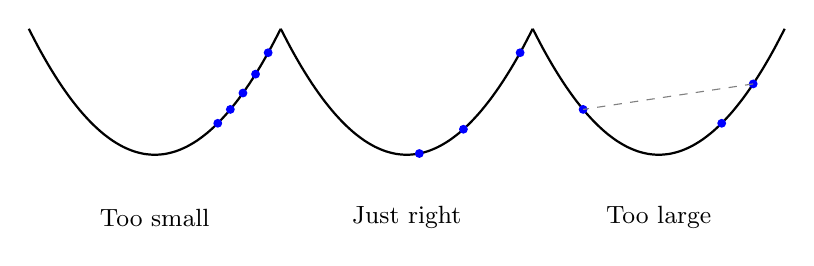
\begin{tikzpicture}[scale=0.8]
    % Small learning rate
    \begin{scope}[shift={(-4,0)}]
        \draw[thick] plot[smooth, domain=-2:2] (\x, {0.5*\x*\x});
        \foreach \x in {1.8, 1.6, 1.4, 1.2, 1.0} {
            \fill[blue] (\x, {0.5*\x*\x}) circle (2pt);
        }
        \node at (0, -1) {\small Too small};
    \end{scope}
    
    % Good learning rate
    \begin{scope}[shift={(0,0)}]
        \draw[thick] plot[smooth, domain=-2:2] (\x, {0.5*\x*\x});
        \fill[blue] (1.8, 1.62) circle (2pt);
        \fill[blue] (0.9, 0.405) circle (2pt);
        \fill[blue] (0.2, 0.02) circle (2pt);
        \node at (0, -1) {\small Just right};
    \end{scope}
    
    % Large learning rate
    \begin{scope}[shift={(4,0)}]
        \draw[thick] plot[smooth, domain=-2:2] (\x, {0.5*\x*\x});
        \fill[blue] (1.5, 1.125) circle (2pt);
        \fill[blue] (-1.2, 0.72) circle (2pt);
        \fill[blue] (1.0, 0.5) circle (2pt);
        \draw[dashed, gray] (1.5, 1.125) -- (-1.2, 0.72);
        \node at (0, -1) {\small Too large};
    \end{scope}
\end{tikzpicture}
\end{center}

% ============================================================================
% VARIANTS
% ============================================================================

\section{Variants of Gradient Descent}

\subsection{Batch Gradient Descent}

Uses the entire dataset to compute the gradient:
\[
\nabla_{\vect{w}} R(\vect{w}) = \frac{1}{N} \sum_{i=1}^{N} \nabla_{\vect{w}} \mathcal{L}(f(\vect{x}_i; \vect{w}), y_i)
\]

\textbf{Pros}: Stable, accurate gradient. \textbf{Cons}: Slow for large datasets.

\subsection{Stochastic Gradient Descent (SGD)}

Uses a single random sample per update:
\[
\vect{w}_{t+1} = \vect{w}_t - \eta \nabla_{\vect{w}} \mathcal{L}(f(\vect{x}_i; \vect{w}_t), y_i)
\]

\textbf{Pros}: Fast updates. \textbf{Cons}: Noisy gradients, erratic convergence.

\subsection{Mini-Batch Gradient Descent}

Uses a small batch of $B$ samples:
\[
\nabla_{\vect{w}} R(\vect{w}) \approx \frac{1}{B} \sum_{i \in \text{batch}} \nabla_{\vect{w}} \mathcal{L}(f(\vect{x}_i; \vect{w}), y_i)
\]

\textbf{The standard choice in practice}: balances efficiency and stability.

\begin{bluebox}[Typical Batch Sizes]
Common mini-batch sizes are powers of 2 (32, 64, 128, 256) for computational efficiency on GPUs. Larger batches give more stable gradients; smaller batches provide regularization through noise.
\end{bluebox}

% ============================================================================
% COMPUTING GRADIENTS
% ============================================================================

\section{Computing Gradients}

\subsection{The Challenge}

For a neural network with millions of parameters, computing $\nabla_{\vect{w}} R(\vect{w})$ efficiently is non-trivial. We need:
\[
\frac{\partial R}{\partial W_{ij}^{[l]}}, \quad \frac{\partial R}{\partial b_i^{[l]}} \quad \text{for all layers } l
\]

\subsection{The Solution: Backpropagation}

\textbf{Backpropagation} is an efficient algorithm for computing gradients in neural networks. It uses the \textbf{chain rule} to propagate error signals backward through the network.

\begin{importantbox}[Key Insight]
Backpropagation is not a learning algorithm---it's a method for efficiently computing gradients. The learning algorithm is gradient descent.
\end{importantbox}

We will derive backpropagation in detail in the next chapter.

% ============================================================================
% IMPLEMENTATION
% ============================================================================

\section{Implementation}

\begin{lstlisting}[language=Python, caption=Gradient Descent Implementation]
import numpy as np

def gradient_descent(X, y, model, loss_fn, learning_rate=0.01, 
                     epochs=1000, batch_size=32):
    """
    Mini-batch gradient descent.
    
    Args:
        X: Training inputs (n_samples, n_features)
        y: Training targets (n_samples,)
        model: Neural network with forward() and backward() methods
        loss_fn: Loss function with gradient
        learning_rate: Step size
        epochs: Number of passes through data
        batch_size: Mini-batch size
    """
    n_samples = X.shape[0]
    losses = []
    
    for epoch in range(epochs):
        # Shuffle data
        indices = np.random.permutation(n_samples)
        X_shuffled = X[indices]
        y_shuffled = y[indices]
        
        epoch_loss = 0
        for i in range(0, n_samples, batch_size):
            # Get mini-batch
            X_batch = X_shuffled[i:i+batch_size]
            y_batch = y_shuffled[i:i+batch_size]
            
            # Forward pass
            y_pred = model.forward(X_batch)
            
            # Compute loss
            loss = loss_fn(y_pred, y_batch)
            epoch_loss += loss
            
            # Backward pass (compute gradients)
            gradients = model.backward(y_pred, y_batch)
            
            # Update parameters
            for param, grad in zip(model.parameters, gradients):
                param -= learning_rate * grad
        
        losses.append(epoch_loss / (n_samples // batch_size))
    
    return losses
\end{lstlisting}

% ============================================================================
% SUMMARY
% ============================================================================

\section{Chapter Summary}

\begin{itemize}
    \item \textbf{Learning objective}: Minimize difference between model and true generating function. Since we don't know the true function, we minimize \textbf{empirical risk} over training data.
    
    \item \textbf{Empirical risk}: $R(\vect{w}) = \frac{1}{N} \sum_{i=1}^{N} \mathcal{L}(f(\vect{x}_i; \vect{w}), y_i)$
    
    \item \textbf{Gradient descent}: Iteratively update parameters in the direction opposite to the gradient:
    \[
    \vect{w}_{t+1} = \vect{w}_t - \eta \nabla_{\vect{w}} R(\vect{w}_t)
    \]
    
    \item \textbf{Learning rate $\eta$}: Critical hyperparameter. Too small = slow; too large = diverge.
    
    \item \textbf{Variants}: Batch (full data), SGD (one sample), Mini-batch (best of both).
    
    \item \textbf{Backpropagation}: Efficient algorithm for computing gradients (next chapter).
\end{itemize}

\begin{bluebox}[Looking Ahead]
We now understand the optimization objective and gradient descent. The remaining question is: \textbf{How do we efficiently compute gradients in deep networks?}

This leads to \textbf{backpropagation}---the subject of our next chapter.
\end{bluebox}
